\documentclass{article}
\usepackage{amsmath}
\usepackage{amssymb}
\usepackage{graphicx}
\usepackage{float}
\begin{document}
	\section{Examples}
	Here are some examples from allaboutcircuits.com.
	\subsection{Example 1}
	Initial values of:
	\begin{itemize}
		\item $R_1, R_2, R_3 = 4, 2, 1 \Omega$
		\item $B_1, B_2 = 28, 7 \text{V}$
	\end{itemize}
	\paragraph[Branch]{Using the Branch Method:}
	There are three unknown currents, each denoted as '$I_1$', '$I_2$', and 
	'$I_3$' respectively.
	\begin{figure}[H]\label{fig:circuit}
		\caption{A complex circuit with two batteries.}
		\centering
		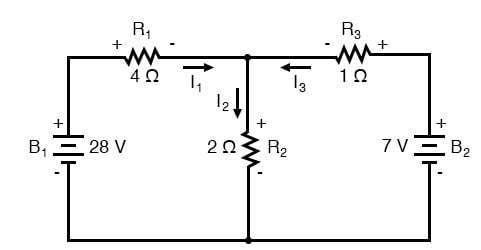
\includegraphics[width=0.75\linewidth,height=0.375\linewidth]{circuit-1}
	\end{figure}
	Note that the polarity of the circuit components are just initial 
	assumptions, which may in fact be incorrect.  These assumptions being 
	incorrect is okay however. \\ \\
	To solve for these unknown values we will use the following three 
	(simultaneous) equations:
	\begin{equation}\label{eq:series_1}
		R_1I_1 + R_2I_2 = B_1
	\end{equation}
	\begin{equation}\label{eq:series_2}
		R_3I_3 + R_2I_2 = B_2
	\end{equation}
	\begin{equation}\label{eq:cur_2-in-cur_1--cur_3}
		I_2 = I_1 + I_3
	\end{equation}
	Equation (\ref{eq:cur_2-in-cur_1--cur_3}) is via Kirschoff's Current 
	Law(KCL), which says that:
	$$ I_1 + I_3 - I_2 = 0\text{A}$$
	Note that the sign (i.e. positive or negative) of a symbol denotes the 
	direction of the current, with respect to the node defined by the 
	connection between the currents, whose measure it represents.  In the case 
	of the above equation, the current with a measure of $I_2$ is 
	\emph{exiting} the node, and, as such, '$I_2$' is preceded by a negative 
	sign in the equation derived from KCL.   $I_1$ and $I_3$ are 
	\emph{entering} the node, which is signified by a lack of a negative sign 
	preceding their symbolic representation in equation 
	(\ref{eq:cur_2-in-cur_1--cur_3}).\\ \\
	Via equation (\ref{eq:cur_2-in-cur_1--cur_3}) and substitution, the first 
	two equations 
	can be rewritten as:
	\begin{equation}\tag{\ref{eq:series_1}}
		R_1I_1 + R_2(I_1 + I_3) = B_1
	\end{equation}
	\begin{equation}\tag{\ref{eq:series_2}}
		R_3I_3 + R_2(I_1 + I_3) = B_2
	\end{equation}
	Via equation (\ref{eq:series_1}), we can solve for $I_1$ in terms of $I_3$.
	$$ I_1(R_1 + R_2) = B_1 - R_2I_3$$
	$$ 6 \Omega \cdot I_1 = 28\text{V} - 2 \Omega \cdot I_3$$
	\begin{equation}\label{eq:cur_1-in-cur_3}
		I_1 = \frac{14}{3}\text{A} - \frac{1}{3}I_3
	\end{equation}
	And, via the above equation, equation (\ref{eq:series_2}), and 
	substitution, we can solve for $I_3$.
	$$ R_3I_3 + R_2 \frac{14\text{A}- I_3 + 3I_3}{3} = R_3I_3 + R_2 
	\frac{14\text{A} + 2I_3}{3} = B_2$$
	$$ 3R_3I_3 + R_2(14\text{A} + 2I_3) = 3B_2$$
	$$ I_3(3R_3 + 2R_2) = 3B_2 - 14\text{A} \cdot R_2$$
	$$ 7\Omega \cdot I_3 = 21\text{V} - 28\text{V} = -7\text{V}$$
	\begin{equation}\label{eq:cur_3}
		I_3 = -1\text{A}
	\end{equation}
	The fact that we got a negative value for $I_3$ implies that our initial 
	assumption about the polarity of $R_3$ was false.  It actually is the 
	opposite, which also means that $I_3$ is in fact \emph{exiting} the 
	node.
	\begin{figure}[H]\label{fig:circuit-2}
		\caption{Same circuit with reversed polarities for $R_3$.}
		\centering
		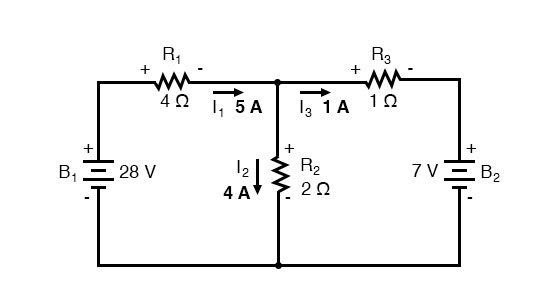
\includegraphics[width=0.75\linewidth,height=0.375\linewidth]{complex-2}
	\end{figure}
	This means that equation (\ref{eq:cur_2-in-cur_1--cur_3})  and 
	(\ref{eq:cur_3}) can be rewritten as:
	\begin{equation}\tag{\ref{eq:cur_3}}
		I_3 = 1\text{A}
	\end{equation}
	$$ I_1-I_2-I_3 =0$$
	\begin{equation}\label{eq:cur_1-in-cur_2}
		I_1 = I_2 + I_3 = I_2 + 1
	\end{equation}
	Note that even if we ignored the polarities and direction of the current 
	altogether, the magnitude of the currents would be the same. \\ \\
	Equations (1), (2), and (4) also need to be rewritten to reflect the new 
	polarity.
	\begin{equation}\tag{\ref{eq:series_1}}
		R_1I_1 + R_2(I_1-I_3) = B_1
	\end{equation}
	\begin{equation}\tag{\ref{eq:series_2}}
		R_3I_3 + R_2(I_1 - I_3) = B_2
	\end{equation}
	\begin{equation}\tag{\ref{eq:cur_1-in-cur_3}}
		I_1 = \frac{1}{3}(14\text{A} + I_3) = \frac{15}{3}\text{A} = 5\text{A}
	\end{equation}
	Finally, via the above equation, equation (\ref{eq:cur_1-in-cur_2}), and 
	substitution,
	$$ I_2 = 5\text{A}-1\text{A}=4\text{A}$$
	\subsection{Example 2}
	Below is a complex circuit that would require 6 branch currents to solve 
	using the branch method.
	\begin{figure}[H]\label{fig:circuit-3}		
		\caption{The Unbalanced Wheatstone Bridge.}
		\centering
		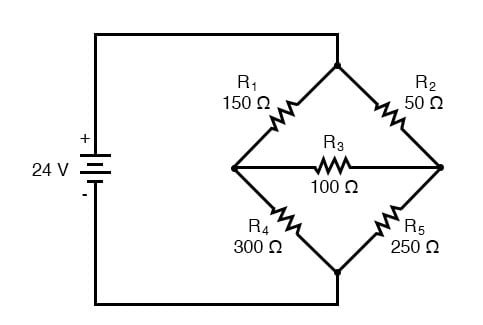
\includegraphics[width=0.75\linewidth,height=0.5\linewidth]{circuit-3}
	\end{figure}
	\subsubsection[Paradigm]{The Paradigm}
	The main paradigm is such that each node, where a node is a connection 
	between two or more circuit wires or links, has an index or subscript.  The 
	top node, denoted as '$N_1$', has an index of one;  The left node: four;  
	Right: two;  And the bottom: three. \\ \\
	A vector with an initial point of $N_1$ and a terminal at $N_2$ may be 
	denoted as either '$\overrightarrow{N_1N_2}$' or '$\overrightarrow{12}$'.  
	If $N_1$ were the default initial point, '$\mathbf{N_2}$' would also be an 
	appropriate denotation for the aforementioned vector, but that is not the 
	case here. \\ \\
	A directed cyclic graph formed by the vectors, $\overrightarrow{N_1N_2}$, 
	$\overrightarrow{N_2N_4}$, and $\overrightarrow{N_4N_1}$ may be denoted as 
	either '$\overrightarrow{N_1N_2N_4N_1}$' or '$\overrightarrow{1241}$'.  
	Mesh currents form a directed cyclic graph and can be denoted the same 
	way;  A mesh current flowing through $R_2$, $R_3$, and $R_1$ in a clock 
	wise direction could be denoted as '$\overrightarrow{N_1N_2N_4N_1}$' or 
	'$\overrightarrow{1241}$'. 
	\paragraph[Current Vector]{The measure of a current} is a vector value;  It 
	has both a magnitude and a direction.  Let $\mathbf{i_2}$ be defined as 
	$\mathbf{i_2}:=\overrightarrow{12}$.  It follows that the magnitude is 
	given 
	by $|\mathbf{i_2}| = \overline{12}$.  The magnitude is of course a scalar 
	value and is always positive.  The direction that the current flows in is 
	arbitrary when it comes to the magnitude of the current.  It also follows 
	that when the sign of a current vector is negative the direction is 
	reversed. 
	$$-\mathbf{i_2}=-\overrightarrow{12}=\overleftarrow{12}=\overrightarrow{21}$$
	In the above equation, the current flows from node 2 to node 1.
	\subsubsection[Mesh]{Mesh Current Method}
	The mesh current method only requires 3 mesh currents to 
	find the 
	currents flowing through each component and subsequently the voltages 
	running across them. \\ \\
	One of these currents, denoted as '$I_1$', flows clockwise through $R_1$, 
	$R_2$, and $R_3$.  Current $I_2$ flows counterclockwise through $R_3$, 
	$R_5$, and 
	$R_4$.  And current $I_3$ also flows clockwise through the battery, denoted 
	as '$B_1$', $R_1$, and $R_4$. \\ \\
	Let $I_1$, $I_2$, and $I_3$ be defined as:
	$$ I_1:=\overrightarrow{1241}$$
	$$ I_2:=\overrightarrow{3423}$$
	$$ I_3:=\overrightarrow{1431}$$
	The assumed polarity of each resistor is such that the positive pole, 
	denoted as '$(+)$', is on the:
	\begin{enumerate}
		\item Left side of $R_1$;
		\item Left side of $R_2$;
		\item Right;
		\item Left;
		\item Left.
	\end{enumerate}
	Via Kirschoff's Voltage Law(KVL),
	\begin{equation}\label{eq:mesh-3}
		24\text{V} - R_1(I_3-I_1) - R_4(I_3-I_2) = 0
	\end{equation}
	\begin{equation}\label{eq:mesh-1}
		R_2I_1 + R_3(I_1-I_2) + R_1(I_1-I_3) = 0
	\end{equation}
	\begin{equation}\label{eq:mesh-2}
		R_3(I_2-I_1) + R_4(I_2-I_3) + R_5I_2 = 0
	\end{equation}
	First, we solve for $I_2$ in terms of the other currents using 
	equation(\ref{eq:mesh-2}).
	$$ R_3I_1+R_4I_3-I_2(R_3 + R_4 + R_5) = 0$$
	\begin{equation}\label{eq:cur_2-in-cur_1-cur_3}
		I_2 = \frac{R_3I_1 + R_4I_3}{650\Omega}
	\end{equation}
	Now we substitute '$I_2$' in equations (\ref{eq:mesh-1}) and 
	(\ref{eq:mesh-3}) with the right hand side of the above equation.
	\begin{equation}\tag{\ref{eq:mesh-3}}
		24\text{V} -R_1(I_3-I_1) - R_4I_3+\frac{6}{13}(R_3I_1 + R_4I_3) = 0
	\end{equation}
	\begin{equation}\tag{\ref{eq:mesh-1}}
		R_2I_1 + R_3I_1-\frac{2}{13}(R_3I_1 + R_4I_3) + R_1(I_1-I_3) = 0
	\end{equation}
	Via equation (\ref{eq:mesh-1}) we can solve for $I_1$ in terms of $I_3$.
	$$ I_1\left(R_2+R_3\frac{11}{13}+R_1 \right)=I_3 \left( R_4 
	\frac{2}{13}+R_1\right)$$
	$$ 284.62I_1 = 196.15I_3$$
	\begin{equation}\label{eq:mesh_1-in-mesh_3}
		I_1 = 0.689 \cdot I_3
	\end{equation}
	Via the above equation, equation (\ref{eq:mesh-3}, and substitution, we can 
	solve for $I_3$.
	$$ 24\text{V} -0.311\cdot R_1I_3 - R_4I_3 + \frac{6}{13}I_3(0.689\cdot 
	R_3+R_4)=0$$
	$$ -24\text{V} = -176.39 \Omega \cdot I_3$$
	\begin{equation}\label{eq:meshcur_3}
		I_3 = 136.06\text{mA}
	\end{equation}
	\begin{equation}\label{eq:meshcur_1}
		I_1 = 93.75\text{mA}
	\end{equation}
	Via equations (\ref{eq:meshcur_1}), (\ref{eq:meshcur_3}), 
	(\ref{eq:cur_2-in-cur_1-cur_3}), and substitution,
	$$ I_2=77.22\text{mA}$$
\end{document}